\documentclass{beamer}
\usetheme{Szeged}
\definecolor{beamer@andja}{rgb}{0.8, 0.4, 0.5}
\setbeamercolor{structure}{fg=beamer@andja}	
\usepackage{beamerthemeshadow}
\usepackage{url}
\usepackage[utf8]{inputenc}
\usepackage{graphicx}

\setbeamertemplate{footline}{\hspace*{.5cm}\scriptsize{\hspace*{50pt} \hfill\hspace*{.5cm}}\\
\vspace{9pt}}

\usepackage[english]{babel}

\begin{document}
\title{\Large InBus\\ \scriptsize {TADHACK 2019}\\ \vspace{15pt}\tiny{ \\}}
\institute {TeleSign\\ }
\author{\scriptsize{Luka Milošević}\\\scriptsize{Stefan Kapunac}\\\scriptsize{Anđelka Milovanović}\\ }
\date{\scriptsize  October 13th, 2019}

\begin{frame}
	\titlepage
\end{frame}
\setbeamertemplate{footline}
{
  \leavevmode
  \hbox{
  \begin{beamercolorbox}[wd=.5
  	\paperwidth,ht=2.25ex,dp=1ex,center]{author in head/foot}
    \usebeamerfont{author in head/foot}{Maheri}
  \end{beamercolorbox}
  \begin{beamercolorbox}[wd=.48\paperwidth,ht=2.25ex,dp=1ex,center]{title in head/foot}
    \usebeamerfont{title in head/foot}{InBus}
  \end{beamercolorbox}}
}

\setbeamertemplate{section in toc}[sections numbered]
\setbeamertemplate{subsection in toc}[subsections numbered]
\setbeamerfont{subsection in toc}{size=\footnotesize}


\section{Introduction} 
\subsection{Example 1}
\begin{frame}\frametitle{Example 1}
\begin{figure}[h!]
   \begin{center}
   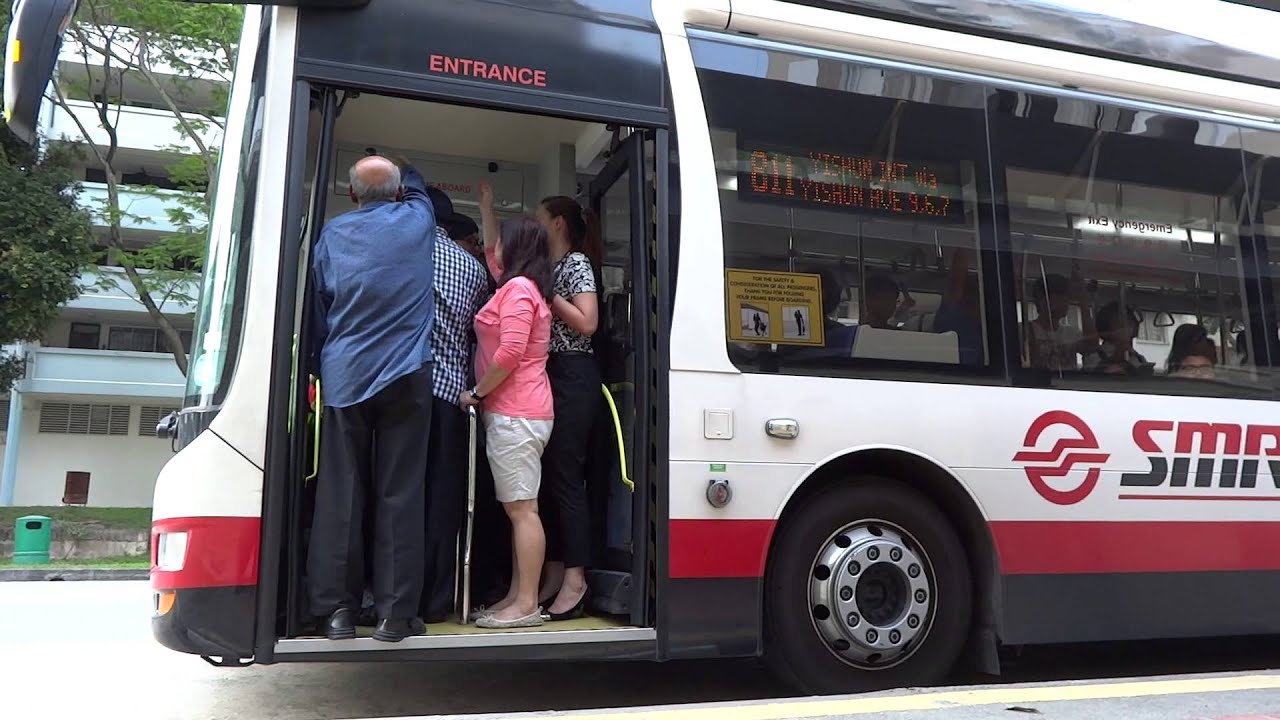
\includegraphics[scale=0.23]{bus.png}
   \end{center}
   \caption{Bus situation}
   \end{figure}
\end{frame}

\subsection{Example 2}
\begin{frame}\frametitle{Example 2}
\begin{figure}[h!]
   \begin{center}
   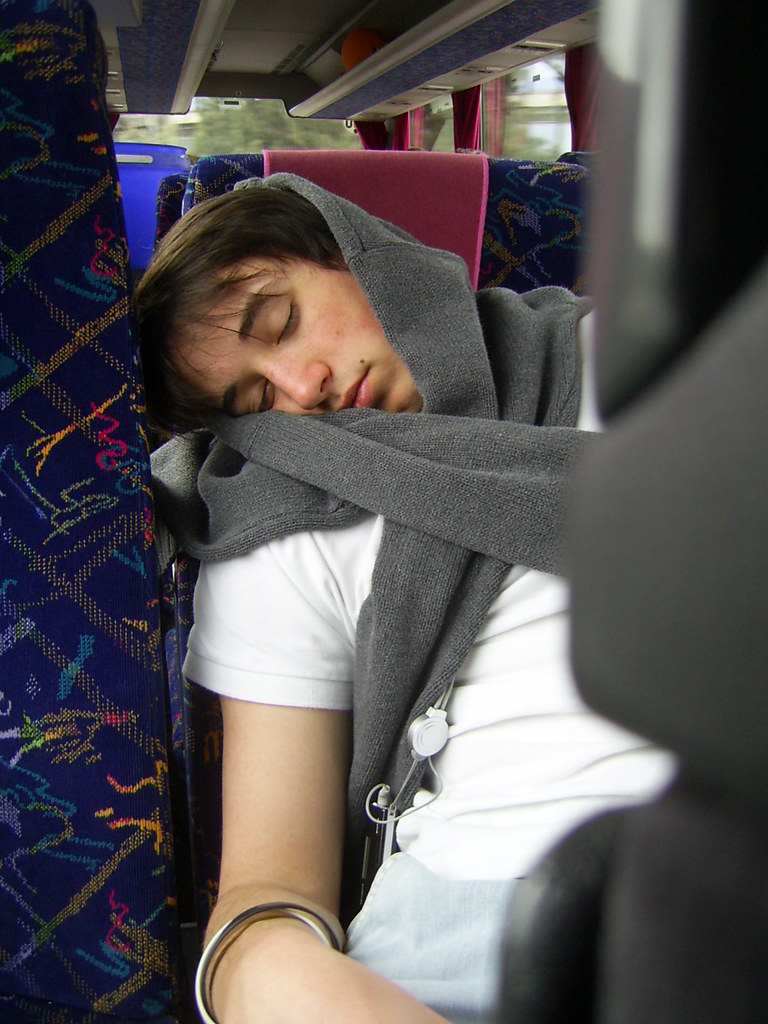
\includegraphics[scale=0.16]{sleep.png}
   \end{center}
   \caption{Sleep situation} 
   \end{figure}
    
\end{frame}

\subsection{Example 3}
\begin{frame}\frametitle{Example 3}
\begin{figure}[h!]
   \begin{center}
   
\includegraphics[scale=0.15]{school_bus.png}
   \end{center}
   \caption{Kids on excursion}
   \end{figure}
    
\end{frame}

\section{Application}
\subsection{InBus}
\begin{frame}\frametitle{Tools}
\begin{itemize}
   \item Android Studio (first ever)
   \item TeleSign API for SMS
   \item Google Maps API
   \item Java
 \end{itemize}    
\end{frame}

\begin{frame}\frametitle{Working App Demo}
   \begin{figure}[h!]
   \begin{center}
   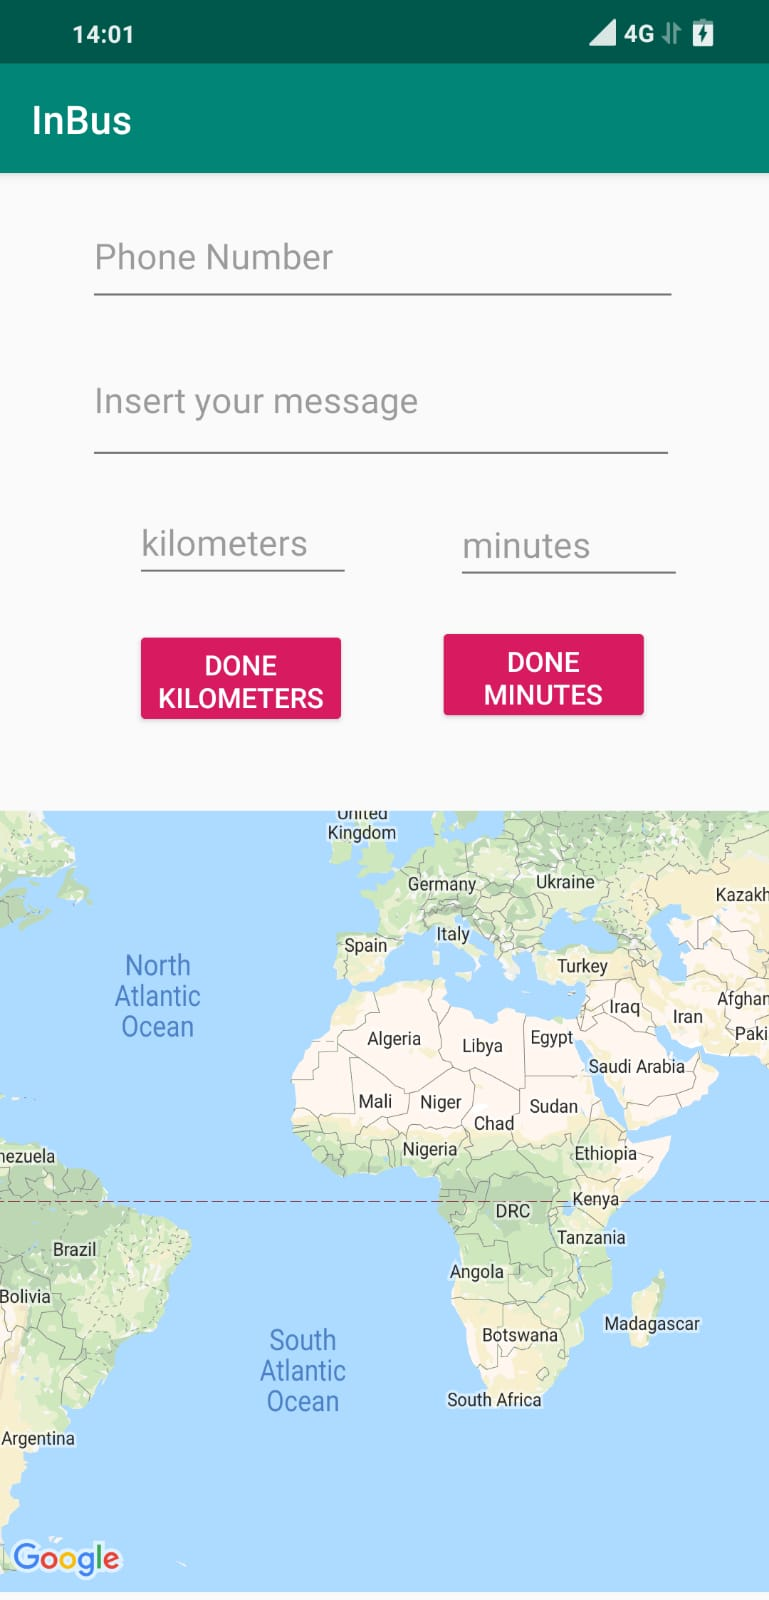
\includegraphics[scale=0.11]{app.jpg}
   \end{center}
   \end{figure}
\end{frame}

\section{Future Extensions}
\begin{frame}\frametitle{Out of Range}
\begin{figure}[h!]
   \begin{center}
   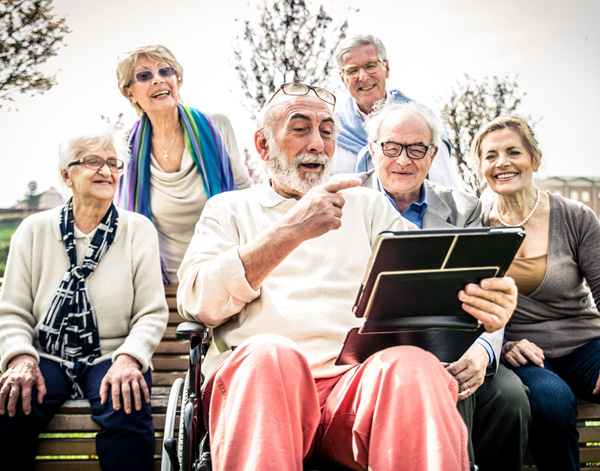
\includegraphics[scale=0.3]{elders.jpg}
   \end{center}
   \caption{Elders}
\end{figure}
\end{frame}

\begin{frame}\frametitle{Reverse problem}
\begin{figure}[h!]
   \begin{center}
   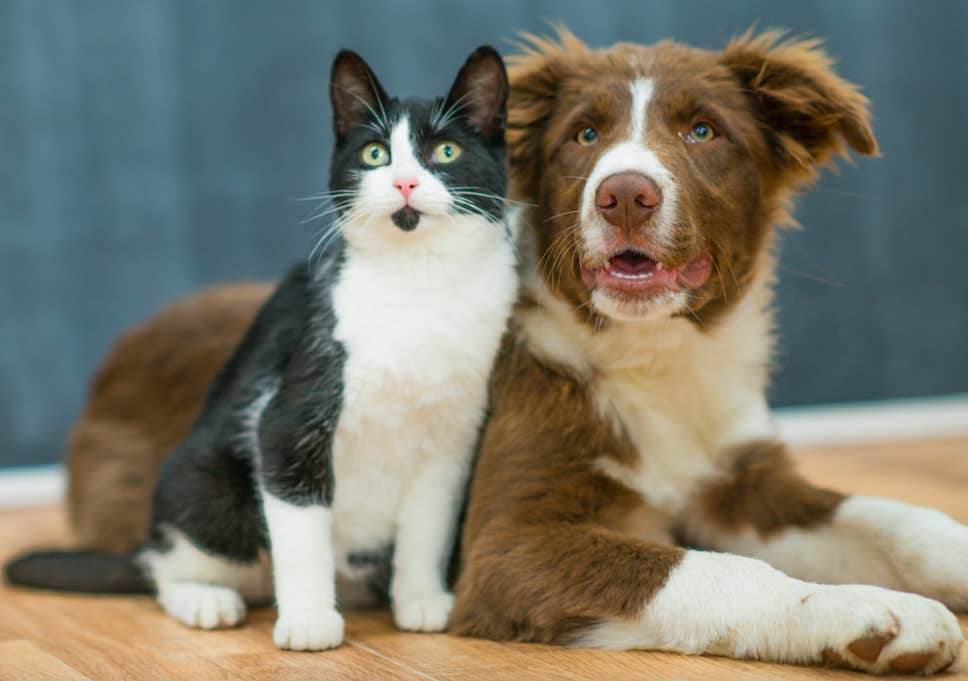
\includegraphics[scale=0.2]{pets.jpg}
   \end{center}
   \caption{Pets}
   \end{figure}
\end{frame}


\section{Questions?}
\begin{frame}
Thank you!
\newline
Questions?
\newline
\vspace{30pt}
\end{frame}

\setbeamertemplate{footline}{\hspace*{.5cm}\scriptsize{\hspace*{50pt} \hfill\hspace*{.5cm} \setbeamercolor{black}}\\
\vspace{9pt}}

\setbeamertemplate{headline}{\hspace*{.5cm}\scriptsize{\hspace*{50pt} \hfill\hspace*{.5cm} \setbeamercolor{black}}\\
\vspace{1pt}}

%\setbeamercolor{mysection in head/foot}{bg= black fg=black}

\end{document}